% Componer (V^i) frente a proyectar (V_i) en la base oblicua a 60° (geometría exacta).
% g1 = (1,0), g2 = (1/2, √3/2), V = (2, 3/2).  V^1 = 2−(3/2)/√3, V^2 = 3/√3;  V_1 = 2, V_2 = 1+3√3/4.
% Compilar con: scripts/compilar_tikz.sh   (→ figures/svg/bases-componer-proyectar.svg)
\def\pgfsysdriver{pgfsys-dvisvgm.def}
\documentclass[tikz,border=4pt]{standalone}
\usetikzlibrary{calc,arrows.meta}
% PALETA-INICIO (generado por scripts/sincronizar_paleta.jl; no editar a mano)
\definecolor{azul}{HTML}{1B6CA8}
\definecolor{naranja}{HTML}{D95F02}
\definecolor{verde}{HTML}{2A9D8F}
\definecolor{gris}{HTML}{6B7280}
\definecolor{violeta}{HTML}{6F42C1}
\definecolor{ocre}{HTML}{8A5A00}
\definecolor{malla}{HTML}{CBD5E1}
% PALETA-FIN
\begin{document}
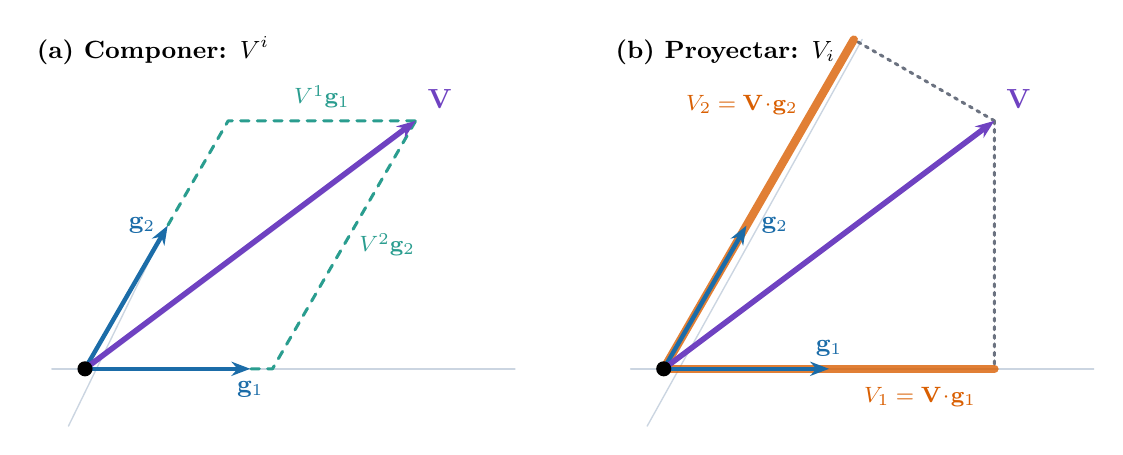
\begin{tikzpicture}[scale=2.1, line cap=round, line join=round, >={Stealth[length=2.4mm]}]
  \pgfmathsetmacro{\rt}{sqrt(3)}
  \pgfmathsetmacro{\vuno}{2-1.5/\rt}
  \pgfmathsetmacro{\vdos}{3/\rt}
  \pgfmathsetmacro{\wdos}{1+3*\rt/4}   % V_2 = V·g2
  % ---------------- (a) Componer: V = V^1 g1 + V^2 g2
  \begin{scope}
    \node[anchor=south west, font=\small\bfseries] at (-0.35,1.78) {(a) Componer: $V^i$};
    \draw[malla, line width=0.5pt] (-0.2,0) -- (2.6,0);
    \draw[malla, line width=0.5pt] (-0.1,{-0.2*\rt}) -- (0.45,{0.9*\rt/2});
    \draw[verde, line width=1.1pt, dashed] (0,0) -- (\vuno,0) -- (2,1.5);
    \draw[verde, line width=1.1pt, dashed] (0,0) -- ({\vdos*0.5},{\vdos*\rt/2}) -- (2,1.5);
    \draw[azul, ->, line width=1.6pt] (0,0) -- (1,0);
    \draw[azul, ->, line width=1.6pt] (0,0) -- (0.5,{\rt/2});
    \node[azul, font=\small, below=1pt] at (1,0) {$\mathbf{g}_1$};
    \node[azul, font=\small, left=1pt] at (0.5,{\rt/2}) {$\mathbf{g}_2$};
    \draw[violeta, ->, line width=2.0pt] (0,0) -- (2,1.5) node[above right] {$\mathbf{V}$};
    \node[verde, font=\footnotesize, above=1pt] at ({(\vdos*0.5+2)/2},{(\vdos*\rt/2+1.5)/2}) {$V^1\mathbf{g}_1$};
    \node[verde, font=\footnotesize, right=2pt] at ({(\vuno+2)/2},{0.75}) {$V^2\mathbf{g}_2$};
    \fill (0,0) circle (1.3pt);
  \end{scope}
  % ---------------- (b) Proyectar: V_i = V·g_i
  \begin{scope}[xshift=3.5cm]
    \node[anchor=south west, font=\small\bfseries] at (-0.35,1.78) {(b) Proyectar: $V_i$};
    \draw[malla, line width=0.5pt] (-0.2,0) -- (2.6,0);
    \draw[malla, line width=0.5pt] (-0.1,{-0.2*\rt}) -- (1.2,{2.3*\rt/2});
    \coordinate (P1) at (2,0);
    \coordinate (P2) at ({\wdos*0.5},{\wdos*\rt/2});
    \draw[gris, dotted, line width=1.1pt] (2,1.5) -- (P1);
    \draw[gris, dotted, line width=1.1pt] (2,1.5) -- (P2);
    \draw[naranja, line width=3pt, opacity=0.8] (0,0) -- (P1);
    \draw[naranja, line width=3pt, opacity=0.8] (0,0) -- (P2);
    \node[naranja, font=\footnotesize, below=3pt] at (1.55,0) {$V_1=\mathbf{V}\!\cdot\!\mathbf{g}_1$};
    \node[naranja, font=\footnotesize, left=3pt] at ({\wdos*0.5*0.8},{\wdos*\rt/2*0.8}) {$V_2=\mathbf{V}\!\cdot\!\mathbf{g}_2$};
    \draw[azul, ->, line width=1.6pt] (0,0) -- (1,0);
    \draw[azul, ->, line width=1.6pt] (0,0) -- (0.5,{\rt/2});
    \node[azul, font=\small, above=1pt] at (1,0) {$\mathbf{g}_1$};
    \node[azul, font=\small, right=2pt] at (0.5,{\rt/2}) {$\mathbf{g}_2$};
    \draw[violeta, ->, line width=2.0pt] (0,0) -- (2,1.5) node[above right] {$\mathbf{V}$};
    \fill (0,0) circle (1.3pt);
  \end{scope}
\end{tikzpicture}
\end{document}
